\chapter{Requirements}
\label{requirements}

The previous discussions overview operators' motivations and practices for pipeline integrity management. We've also covered the geographic and technological framework that RAPID works within---primarily adhering to OGC's Abstract Specification. Alongside external pipeline operating partners, our team established additional requirements for RAPID's domain-specific functionality.

At a high level, our goal is to combine the earlier-mentioned spatial operations and formats with updatable and searchable  geographic data. Partner organizations also require permissioning capabilities so that private and proprietary information is not shared with unprivileged requesters.

These broad characteristics are spelled out below, and we describe the subsequent system design for meeting these requirements in Chapter~\ref{design}.\footnote{Of additional note, these requirements are particularly suited to RAPID's \textit{data model}. Other tertiary requirements exist for the REST API---pertaining to its style and usage---but many of those are derived from the central asks in this chapter. Francis's thesis describes the API's requirements and design in depth~\cite{Francis}.}

\section{Input formats}

Throughout our own experimentation and research, GeoJSON and Shapefiles (both summarized in Chapter~\ref{background}) emerged as reasonable starting points for file importing in RAPID. There are several reasons:

\begin{description}
  \item[Availability.] Many (or even most) high-profile, public geospatial datasets are archived in one or both of these formats.
  \item[Standardization.] While not wholly formulated by the OGC, both GeoJSON and Shapefiles incorporate the Abstract Specification, and other components of the formats are open standards. This, in part, drives their ubiquity and availability.
  
Shapefiles, primarily Esri's creation for their ArcGIS software, include many standard \textit{and} non-standard amendments and appendages. While some of these are used to enable extended functionality in proprietary systems, they're often used for (optional) performance tuning. That is, the most essential vector data is openly specified, and the other components aren't particularly important to us.

\item[Toolsets.] Thanks to their standardization and popularity, these formats  are well-supported by many open-source spatial libraries and frameworks. This means a lot of robust, reusable functionality for parsing and validation already exists.

\item[Abstraction and conversion.] Again, with the consideration that these vector formats are standardized and built on top of the Abstract Specification, their data types can store and represent the \textit{same information}.

Further, these representations can be converted from one to another: the vectors of a valid GeoJSON file can be entirely converted to a Shapefile with the same vectors. This also means that end users---even third party developers---don't often need to know the underlying detail of which file format was used at one point or another. In the case that one particular format is required, the conversion is mostly trivial.

\item[GeoJSON readability and ubiquity.] GeoJSON's relatively user-friendly and readable syntax (extended from JSON) lets nontechnical stakeholders and contractors understand (and even generate) structured geospatial data with minimal training.

Additionally, the JSON component of GeoJSON particularly suits it for other programming tasks (and software that's not necessarily in the GIS space). Many other formats are only known and initially usable by geospatial professionals, but JSON is accessible for a large portion of developers.

\end{description}

\section{Output formats}
For the same reasons that we settled on GeoJSON and Shapefiles as input formats, they both made sense as output formats, and data in RAPID can be exported as either (no matter the input format).\footnote{This decision was helpful as a practical matter, too: with the tools and libraries we're using, it's less difficult to export formats we've already researched and configured for decoding.} While a commercial, enterprise-ready application might implement several extensive OGC standards for data exchange and parsing---enabling instant plug-and-play functionality for some GIS---GeoJSON, supplemented by Shapefiles, was chosen as a reasonable starting point. It's also not difficult to find open-source libraries that convert these formats to other OGC-compliant ones.\footnote{This functionality could be added to RAPID; it just doesn't exist yet.}

\subsection{Related work and standards}
\subsubsection{Web Feature Service}
OGC's Web Feature Service (WFS) is a lengthy and highly-specific standard for geospatial data storage, formatting, and transmission. Several existing reference implementations also exist. While this complex, in-use standard outdoes RAPID's capabilities in some scenarios, there's currently no standard specification for spatial REST APIs.

This gives Francis and me the opportunity to create the ecosystem that we see fit---even allowing non-GIS developers to incorporate RAPID data relatively pain-free. Our validation software, PolyView,\footnote{Introduced in Section~\ref{polyview_intro} and detailed in~\ref{polyview_details}.} for instance, would not have the resources to interface with a WFS directly, but can still make use of RAPID because of its idiomatic REST API.

\subsubsection{FeatureServer}

One related system we're aware of, a 2013 open-source project called FeatureServer, implements many OGC standards, allowing for automated and full-featured data querying---even adding a REST API for some use cases.

To clarify the difference between FeatureServer and RAPID, though: FeatureServer expects users (developers) to have a thorough understanding of these specific OGC standards, and it acts mostly as a set of helper tools for customers already working amongst those standards. While FeatureServer is a sort of stepping stone between GIS and WFSs, RAPID is lighter-weight and focuses on gathering and publicizing real data, even when it may not end up in a commercial GIS.


\section{Data layers}
\label{reqs_layers}
As we've discussed, the core geographic data model, with geometries and arbitrary properties, is mostly standardized. RAPID begins to differentiate itself with how data is grouped and queried: it's a requirement to have ``layers'' of data, collecting features within user-defined categories---think categorization of weather stats versus census numbers.\footnote{In practice, we don't dictate how to separate layers logically or assign their metadata, but the concept of disparate (but grouped) data is central to RAPID's functionality.}

\paragraph{Example.}
Every five minutes, the United States Geological Survey (USGS) publishes a GeoJSON file on their website of earthquakes from around the world---locations, magnitudes, depths, and such. If RAPID retrieves data at the same five-minute refresh rate, after some hours, it can process tens of GeoJSON input files from the USGS containing hundreds of spatial seismic measurements, all slotted into the same ``earthquake'' category, or \textit{layer}.

While visible under the hood, RAPID won't externally reveal which features came from which files. Even data fetched from several different sources is, effectively, merged (e.g. a pipeline operator could have more granular seismic data alongside the USGS feed); from then on out, all the data is accessible through one uniform, queryable layer.

\subsection{Updatability}
In the previous example, we alluded to RAPID's data modification capabilities and the expectation to regularly and automatically retrieve new data. Existing data sets---layers---need to seamlessly integrate new measurements as they become available.

Similarly, stored data should be modifiable at the feature level through the API; users and applications shouldn't have to edit and resubmit whole Shapefiles or GeoJSON files to slightly tweak the database. In this way, the procedure is programmable and allows for fine-grained manipulation when necessary.

\section{Querying}

Introduced in~\ref{reqs_layers}, RAPID must be programmatically queryable (for the sake of external DSSs), fetching subsets of spatial data filtered by layer, location, and time.

Layers in RAPID can be further characterized by this querying process. In most cases, data from a single layer will be analyzed similarly or aggregated. If a pipeline operator DSS seeks rainfall trends (for example), every feature in RAPID's designated rainfall layer can be returned, and the relevant information is available for study.

For efficiency's sake and user-friendliness, RAPID can offload, from external software, ``cropping'' of data by time and region. That is, users have the option to specify a sub-area and timeframe for data export.

OGC's Simple Features Access, introduced in Chapter~\ref{background}, describes standardized queries for spatial data. Each boolean relational operator (Within, Contains, Intersects, etc.) can be used to filter data, including or excluding features based on the selection criteria.

Refer back to Chapter~\ref{background} for specific examples of GDBMS table selections and joins, but consider RAPID's common use case: the system will gather, export, and transfer recent geographic features for a defined space (represented as a Polygon). Features within\footnote{``Within'' is a technical term---a function---in Simple Features Access, but we aren't using it as such here. We simply mean to designate features contained by or encroaching on the specified region.} by the Polygon and in the correct time period are processed and returned to requestors.

\subsection{Monitored regions}
We solidify the concept of queryable view subsets by making them nameable and saveable. Our design later calls these stored, on-demand filters \textit{GeoViews}.

\begin{figure}
    \centering

    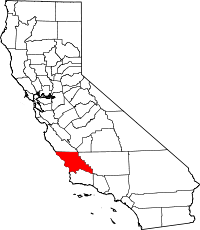
\includegraphics[width=0.3\textwidth]{figures/slo_county.png}
    
    \caption{Borders for San Luis Obispo County, California}
    \label{fig:county}
    
\end{figure}

\paragraph{Example.}
A GeoView for San Luis Obispo (SLO) County, California could be created to retrieve construction info and traffic densities. It's easy to come up with SDSS analyses: pipelines near construction equipment (representable as points) or dense traffic (representable as weighted linestrings) are susceptible to undesired and compromising human contact.\footnote{We assume users have already configured RAPID to gather construction and traffic data; however, notice that the geographical spread of data isn't particularly important at this time.}

To create this GeoView, an analogous Polygon to the county borders in Figure~\ref{fig:county} can be passed to RAPID, along with an identifier for each desired layer. We'll call the GeoView ``SLO Human Factors''---also stored in RAPID for indexing and retrieval.

Any time a requesting user or DSS looks to analyze these local features, they simply query RAPID for the SLO Human Factors GeoView and, optionally, include a start and end time for data. Any points or linestrings from the traffic and construction layers \textit{in SLO County} (and in the optional timespan) are compiled into GeoJSON or Shapefiles and returned to the API caller.

\section{Permission management}
Although RAPID's marquee feature is gathering and sharing data from multiple (and discrete) sources, open and total access discourages organizations from storing and querying their sensitive or trade-secret data. Because aggregating and efficiently filtering this data \textit{is} a requirement for our pipeline operating partners, RAPID must include permission management capabilities for layers and GeoViews, allowing decision-makers to hide information when appropriate.

RAPID's permission model is not overly complicated, but it does have to be precise and secure. In broad terms, layers require Owners that decide their visibility for other users. Non-Owners can be made Viewers or Editors for accessing or modifying data, respectively. This lets users specify which other users can work with layers they create; RAPID provides authentication capabilities for these users and ensures requesters and curators operate within assigned privileges. Layers that are not sensitive in nature and need to otherwise be widely-accessible may be specified as \textit{public} layers.

Chapter~\ref{design} explains the permissioning system we developed in further detail.

\section{Modularity and abstraction}
While this is not an explicit technical requirement, the system architecture should be modular---easily-maintainable with concerns separated. This is for a few reasons:

RAPID will likely see further development in the next several years with different software engineers and stakeholders. While the current RAPID system is a powerful tool for many geospatial operations, we recognize the demand for a broader platform of data aggregation, monitoring, and retrieval, allowing more extensive features down the road.

Ideally, more advanced functionality will fit directly into the models and workflows we've already created; when it doesn't, the RAPID codebase still must be flexible enough to incorporate new work without entirely dismantling existing features and recreating large components from scratch.

From discussions with external partners, we've heard that potential add-ons could be support for additional file formats or even encryption. New developers should be able to join the project, understand the system design quickly, and then add features like these wherever they most belong.

% NEW BELOW
Our design decisions specifically aim for flexibility, clarity, and robustness, as there might be further development in the works for RAPID.